\documentclass[titlepage,a4paper]{article}
\usepackage[T1]{fontenc}		% font encode
\usepackage[utf8]{inputenc}	 % input encode
\usepackage[english]{babel}		% secondary and main languages
\usepackage{authblk}			% to add affiliation
\usepackage[tt]{titlepic}		% to add the logo in first page
\usepackage{graphicx}			% to add images
\usepackage{gensymb}			% used for symbols as °(\degree)
\usepackage{amsmath}
\usepackage{mathtools}			% used for math formulae
\usepackage{float}
\usepackage{titlesec}			%used to add \sectionbreak command
\usepackage{appendix}
\usepackage{hyperref}
\usepackage{footnote}
\usepackage{enumitem}
\usepackage{blindtext}
\usepackage{graphicx}
\usepackage{caption}
\usepackage{subcaption}
\usepackage{listings}
\usepackage{xcolor}
\usepackage{hyperref}
\usepackage{rotating}
\usepackage{siunitx}
\usepackage{textcomp}
\usepackage{listings}		%code listings (lstlisting)
\usepackage{color}

\setlistdepth{9}									% enumerate depth 
\newlist{req_enum}{enumerate}{9}					% definition of a new enumerate type
\setlist[req_enum]{label=\thesubsection.\arabic{*}.}	% include the chapter number

\definecolor{gray}{rgb}{0.4,0.4,0.4}
\definecolor{darkblue}{rgb}{0.0,0.0,0.6}
\definecolor{cyan}{rgb}{0.0,0.6,0.6}

\lstset{basicstyle=\ttfamily,columns=fullflexible,showstringspaces=false,tabsize=2}

\lstdefinestyle{custompython}{backgroundcolor=\color{white},belowcaptionskip=1\baselineskip,breaklines=true,frame=L,xleftmargin=\parindent,language=Python,showstringspaces=false,basicstyle=\footnotesize\ttfamily,keywordstyle=\bfseries\color{darkblue},commentstyle=\itshape\color{green!40!black},identifierstyle=\color{blue},stringstyle=\color{orange},
}


\lstdefinestyle{custombash}{basicstyle=\color{white},backgroundcolor=\color{black},belowcaptionskip=1\baselineskip,breaklines=true,frame=L,xleftmargin=\parindent,language=bash,showstringspaces=false,morekeywords={roslaunch,rosrun},basicstyle=\footnotesize\ttfamily,keywordstyle=\bfseries\color{yellow},commentstyle=\itshape\color{green},identifierstyle=\color{white},stringstyle=\color{orange},
}


\lstdefinelanguage{XML}{morestring=[b]", morestring=[s]{>}{<}, stringstyle=\color{red}, identifierstyle=\color{darkblue}, commentstyle=\color{green}, keywordstyle=\color{cyan}, morekeywords={name,xmlns,version,type}% list your attributes here
}

\newcommand{\sectionbreak}{\clearpage}	%to start new section in a new page

\graphicspath{{img/}{img/Johnny/}{img/rob/screenshots/}}

\renewcommand\Authfont{\fontsize{12}{14.4}\selectfont}
\renewcommand\Affilfont{\fontsize{10}{10.8}\selectfont}

%intestazione
\title{
\includegraphics[width=4cm, keepaspectratio]{unipi_blu}\hspace{2cm}
\includegraphics [width=4cm, keepaspectratio]{santanna}~\\[2cm]
\textbf{\LARGE Design of Embedded Systems}\\[1cm]
ESSTA, Energy Saving Smart-home distributed Temperature control Application\\[1cm]
Requirements}

\author{\emph{Falzone Giovanni}}
\affil{\emph{jointly M.Sc Embedded Computing Systems}}
\affil{\emph{Sant'Anna School of Advanced Studies}}
\affil{\emph{University of Pisa}}

\begin{document}
\maketitle
\tableofcontents

\section{Introduction}
The purpose of this project is to realize a smart-home application to control the heating system of a building based on the temperature of each room, in order to minimize the consumption of the building each room apply an energy saving function reducing the desired temperature when it is not needed.
The system is composed by two differ modules
\begin{itemize}
	\item central unit module 
	\item room module
\end{itemize}

\subsection{Central Unit}
The \textit{Central Unit} has the role of coordinator that retrieve the status of each room and computes the average values for the building.\\

\subsubsection{Graphical user interface}
Using a graphical User Interface the module represents the average values of the building and the values for each room, the graphical User Interface is composed by:
\begin{itemize}
	\item \textit{Main page} to represent the overview of the building
	\item \textit{Room page} to represent the status of each room
	\item \textit{Settings page} to set the desired temperature
\end{itemize}

Whenever the \textit{Main page} is selected the module shall represent the average values among all the rooms for \textit{Temperature}, \textit{Humidity} and \textit{Usage}.\\
Whenever the \textit{Main page} is selected the module shall represent the \textit{Energy Saving} if at least one room is set to \textbf{Energy Saving mode}.\\
Whenever the \textit{Main page} is selected the module shall represent the \textit{Warning} if at least one room is set to \textbf{crashed}.\\
Whenever the \textit{Main page} is selected the module shall allow the user to move in the \textit{Settings page}, next and previous \textit{Room page}.\\

Whenever the \textit{Settings page} is selected the module shall represent the \textit{Desired Temperature} and shall allow the user to increase or deacrease it by a factor of 0.5 C\degree in the range of 15 C\degree and 30 C\degree.\\
Whenever the \textit{Settings page} is selected the module shall represent the average values among all the rooms for \textit{Humidity} and \textit{Usage}.\\
Whenever the \textit{Settings page} is selected the module shall represent the \textit{Energy Saving} if at least one room is set to \textbf{Energy Saving mode}.\\
Whenever the \textit{Settings page} is selected the module shall represent the \textit{Warning} if at least one room is set to \textbf{crashed}.\\
Whenever the \textit{Settings page} is selected the module shall allow the user to move in the \textit{Main page}.\\

Whenever the \textit{Room page} is selected the module shall represent the average values among all the rooms for \textit{Temperature}, \textit{Humidity} and \textit{Usage}.\\
Whenever the \textit{Room page} is selected the module shall represent the \textit{Energy Saving} if at least one room is set to \textit{Energy Saving mode}.\\
Whenever the \textit{Room page} is selected the module shall represent the \textit{Warning} if at least one room is set to \textbf{crashed}.\\
Whenever the \textit{Room page} is selected the module shall allow the user to move in the \textit{Main page}, \textit{Settings page}, next and previous \textit{Room page}.\\

The graphical user interface shall represent the following information as reported in the table \ref{tab:GraphicalInformations}.
\begin{table}[H]
	\centering
			\begin{tabular}{||l | l||} 
			\hline
			\textbf{Information}	& \textbf{Format} \\ 
			\hline
			Temperature	& C\degree \\ 
			\hline
			Humidity	& \% \\ 
			\hline
			Usage		& \% \\ 
			\hline
			Energy Saving	& boolean \\ 
			\hline
			Warning		& boolean \\ 
			\hline
		\end{tabular}
		\captionof{table}{Display Information\label{tab:GraphicalInformations}}
\end{table}

\subsubsection{Communication}
Whenever a \textit{Room Request message} is sent and the \textit{Room Status message} is not received within 20s the module shall mark the room as \textbf{crashed}.
The module shall send the \textit{Room Request message} for each room at least every 30s.

%--------------------------------------
\subsection{Room Module}
The purpose of this module is to control the temperature of the room acting on a valve in order to 
reach and maintain the \textit{GoalTemperature}.

\subsubsection{Energy Saving mode}
In order to minimize the consumption the module keep tracks of the presence of motion inside the room
using a motion sensor. \\

If a motion is detected in the last 30s, the module shall set the \textit{GoalTemperature} to the one set by the user,otherwise the module shall set the \textit{GoalTemperature} to:

\begin{equation}
	GoalTemperature = DesiredTemperature - EnergySavingTemperatureOffset
\end{equation}
Whenever the module is in \textit{Energy Saving mode} it shall notify it through the \textit{Interface}.

\subsubsection{Valve control}
In order to control the heating of the room the valve is moved to different positions based on the temperature error 
(\textit{ActualTemperature} - \textit{GoalThemperature}) as in the following table, 
whenever one of these rules is valid the module shall move the valve in the correspondent position described in the third column of the table \ref{tab:ValvePositions} as percentage of maximum flow.
\begin{center}
	\begin{tabular}{| l | l | l |} 
		\hline
		\textbf{rule} & \textbf{valve position} & \textbf{Flow in \%}\\
		\hline
		\begin{math} error < -HIGH \end{math} &  OPEN\_POSITION & 100\\
		\hline
		\begin{math} error \in [-HIGH, -APPROCHING) \end{math}  & HIGH\_POSITION & 75\\
		\hline
		\begin{math} error \in [-APPROCHING, +APPROCHING] \end{math} & MIDDLE\_POSITION & 50 \\
		\hline
		\begin{math} error \in (APPROCHING, HIGH] \end{math} & LOW\_POSITION & 25\\
		\hline
		error > HIGH &  CLOSED\_POSITION & 0 \\
		\hline
	\end{tabular}
	\captionof{table}{\label{tab:ValvePositions}}
\end{center}
Whenever the valve is in \textit{OPEN\_POSITION} or \textit{CLOSED\_POSITION} the module shall check the position and set \textbf{Valve Error} if it is not valid.

In the following table\ref{tab:TemperatureThresholds} are reported the temperature thresholds:
\begin{center}
	\begin{tabular}{||l | l||} 
		\hline
		HIGH 		& 2 C\degree \\ 
		\hline
		APPROCHING 	& 1 C\degree \\ 
		\hline
	\end{tabular}
	\captionof{table}{\label{tab:TemperatureThresholds}}
\end{center}


\subsubsection{Communication}
Whenever a \textit{Room Request message} is not received within 60s the module shall send the \textit{Room Status Message} and set the \textbf{Communication error}.

\subsubsection{Errors}
Whenever one of the errors are set, the module shall notify it through the \textit{Interface}.
In the following table \ref{tab:RoomErrors} are reported the possible errors.
\begin{center}
	\begin{tabular}{|| l ||} 
		\hline
		\textbf{Valve error} \\ 
		\hline
		\textbf{Communication error} \\ 
		\hline
		\textbf{Sensor error} \\ 
		\hline
	\end{tabular}
	\captionof{table}{\label{tab:RoomErrors}}
\end{center}

\section{Requirements}
	\subsection{Central Unit Data Dictionary}
		\subsubsection{Events}
			\begin{center}
				\resizebox{\textwidth}{!}{\begin{tabular}{|| c | c | c | c| c | c | c | c ||} 
					\hline
					\textbf{Signal  Name} 		& \textbf{Description}	& \textbf{Direction} &\textbf{Trigger}	& \textbf{Data Type} 			& \textbf{Min}		& \textbf{Max}	& \textbf{Unit} \\ 
%------------------------------- User Interface input----------------------------
					\hline
					B\_NEXT 			& Next page	button						& input &	rising	&	Boolean 								& 0					& 1 & \\ 
					\hline
					B\_PREVIOUS			& Previous page button					& input &	rising	&	Boolean 								& 0					& 1 & \\ 
					\hline
					B\_SETTINGS			& Settings button						& input &	rising	&	Boolean 								& 0					& 1 & \\ 
					\hline
					B\_PLUS				& Plus button							& input &	rising	&	Boolean 								& 0					& 1 & \\ 
					\hline
					B\_MINUS 			& Minus button							& input &	rising	&	Boolean 								& 0					& 1 		& \\ 
					\hline

%-----------------------------Room Request message --------------------
					PollingRoomId		& Id of the room displayed				& Output & 				&	Real Positive 						& 1					& 8		 	&   \\ 
					\hline
					DesiredTemperature	& Desired Temperature set by the user	& Output & 				&	Real Positive 						& 15.00				& 30.00	 	& Celsius\degree \\ 
					\hline
%-----------------------------Room Status message --------------------
					RoomId				& Id of the room 						& Input & 				&	Real Positive 						& 1					& 8		 	&   \\ 
					\hline
					RoomTemperature		& Average Temperature of the building	& Input & 				&	Real Positive 						& 15.00				& 30.00		& Celsius\degree \\ 
					\hline
					RoomHumidity		& Average Humidity of the building		& Input & 				&	Real Positive 						& 0.00				& 100.00	& \%	 \\ 
					\hline
					RoomValve			& Average Usage of the building			& Input & 				&	Natural 							& 0					&	100 	&	\%	 \\ 
					\hline
					RoomEco				& Eco status of the building			& Input & 				&	Boolean								& 0					&	1 		&		  \\ 
					\hline
					RoomWarning			& Warning of the building 				& Input & 				&	Boolean								& 0					&	1 		&		  \\ 
					\hline

				\end{tabular}}
			\end{center}

	\subsubsection{Parameters}
		\begin{center}
			\resizebox{\textwidth}{!}{\begin{tabular}{||c | c | c | c | c | c | c ||} 
				\hline
				\textbf{Data} 		& \textbf{Description}					& \textbf{Data Type} 	& \textbf{Min}	& \textbf{Max}	& \textbf{Unit} 	&\textbf{Default}\\ 
				\hline
				POLLING\_PERIOD		&	period for requesting room' status	&	Real Positive 		& 0				& 30 		& Seconds				& 5 \\ 
				\hline
				BuildingTemperature	& Average Temperature of the building	& 	Real Positive 		& 0				& 1 		& Celsius\degree 		& 0 \\ 
				\hline
				BuildingHumidity	& Average Humidity of the building		&	Real Positive 		& 0.00			& 100.00	& \%	 				& 0 \\ 
				\hline
				BuildingUsage		& Average Usage of the building			&	Natural 			& 0				&	100 	&	\%	 				& 0 \\ 
				\hline
				BuildingEco			& Eco status of the building			&	Boolean				& 0				&	1 		&		 				& 0 \\ 
				\hline
				BuildingWarning		& Warning of the building 				&	Boolean				& 0				&	1 		&		 				& 0 \\ 
				\hline
				SelectedRoomId		& Id of the displayed room 				&	Natural 			& 1				&	8 		&		 				& 0 \\ 
				\hline

			\end{tabular}}
		\end{center}

%-----------------------------------------------------------------------------------------

	\subsection{Central Unit Requirements}
		\begin{req_enum}
			\item \textbf{Graphical User Interface}
			\begin{req_enum}[label*=\arabic*.]
					\item \textbf{Main Page}
						\begin{req_enum}[label*=\arabic*.]
							\item \textbf{During}
								\begin{req_enum}[label*=\arabic*.]			
									\item If at least one room is set to \textbf{Energy Saving mode} then the module shall set to true the \textit{BuildingEco} false otherwise \\
									\item If at least one room is marked as \textbf{crashed} the module shall set to true the \textit{BuildingWarning} false otherwise \\
	
									\item If the \textit{Next page} event is set the module shall move in the \textit{Room page} and set the \textit{SelectedRoomId} to the lowest Id among the initialized rooms \\
									\item If the \textit{Previous page} event is set the module shall move in the \textit{Room page} and set the \textit{SelectedRoomId} to the greatest Id among the initialized rooms \\
									\item If the \textit{Settings page} event is set the module shall move in the \textit{Settings page} \\

									\item The module shall represent the \textit{BuildingTemperature} in Celsius\degree \\
									\item The module shall represent the \textit{BuildingHumidity} in \% \\
									\item The module shall represent the \textit{BuildingUsage} \\
									\item The module shall represent the \textit{BuildingEco} and \textit{BuildingWarning} as boolean \\
								\end{req_enum}
						\end{req_enum}

					\item \textbf{Settings Page}
						\begin{req_enum}[label*=\arabic*.]
							\item \textbf{Entry}
							\begin{req_enum}[label*=\arabic*.]
								\item The module shall represent the \textit{plus} and \textit{minus} buttons to allow the user to change the \textit{DesiredTemperature} \\
							\end{req_enum}	
							\item \textbf{During}
							\begin{req_enum}[label*=\arabic*.]
								\item If at least one room is set to \textbf{Energy Saving mode} then the module shall set to true the \textit{BuildingEco} false otherwise \\
								\item If at least one room is marked as \textbf{crashed} the module shall set to true the \textit{BuildingWarning} false otherwise \\

								\item If the \textit{B\_NEXT} event is set the module shall move in the \textit{Room page} and set the \textit{SelectedRoomId} to the lowest Id among the initialized rooms \\
								\item If the \textit{B\_PREVIOUS} event is set the module shall move in the \textit{Room page} and set the \textit{SelectedRoomId} to the greatest Id among the initialized rooms \\
								\item If the \textit{B\_SETTINGS} event is set the module shall move in the \textit{Main page}
								\item If the \textit{B\_PLUS} event is set the module shall increase the \textit{DesiredTemperature} by a factor of 0.5 Celsius\degree if it not exceed the MAX\_TEMPERATURE
								\item If the \textit{B\_MINUS} event is set the module shall decrease the \textit{DesiredTemperature} by a factor of 0.5 Celsius\degree if it is not less then MIN\_TEMPERATURE

								\item The module shall represent the \textit{DesiredTemperature} in Celsius\degree \\
								\item The module shall represent the \textit{BuildingHumidity} in \% \\
								\item The module shall represent the \textit{BuildingUsage} \\
								\item The module shall represent the \textit{BuildingEco} and \textit{BuildingWarning} as boolean \\
							\end{req_enum}
							\item \textbf{Exit}
							\begin{req_enum}[label*=\arabic*.]
								\item The module shall hide the \textit{plus} and \textit{minus} buttons
							\end{req_enum}	
						\end{req_enum}

					\item \textbf{Room Page}
						\begin{req_enum}[label*=\arabic*.]
							\item \textbf{During}
							\begin{req_enum}[label*=\arabic*.]
								\item If the \textit{B\_NEXT} event is set the module shall move in the \textit{Room page} and set the \textit{SelectedRoomId} to the next greater Id among the initialized rooms, if no rooms are available then shall move in the \textit{Main page} \\
								\item If the \textit{B\_PREVIOUS} event is set the module shall set the \textit{SelectedRoomId} to the previous Id among the initialized rooms, if no rooms are available then shall move in the \textit{Main page} \\
								\item If the \textit{B\_SETTINGS} event is set the module shall move in the \textit{Settings page}

								\item The module shall represent the Temperature of the \textit{SelectedRoomId} in Celsius\degree \\
								\item The module shall represent the Humidity of the \textit{SelectedRoomId} in \% \\
								\item The module shall represent the Usage of the \textit{SelectedRoomId} \\
								\item The module shall represent if the \textit{SelectedRoomId} is in \textbf{Energy saving mode} or \textbf{Normal mode} \\
								\item The module shall represent if the \textit{SelectedRoomId} is considered \textbf{Crashed} or not\\
							\end{req_enum}
						\end{req_enum}
					\end{req_enum}
%-----------------------------------------------------
			\item \textbf{Communication}
				\begin{req_enum}[label*=\arabic*.]
					\item \textbf{Entry}
						\begin{req_enum}[label*=\arabic*.]
							\item The module shall send the \textit{InitialMessage} in broadcast
						\end{req_enum}	
					\item \textbf{During}
						\begin{req_enum}[label*=\arabic*.]
							\item The \textit{Central Unit} shall send a \textit{Room Request message} with the \textit{PollingRoomId} and the \textit{DesiredTemperature} in Celsius\degree every POLLING\_PERIOD  \textpm 1 second
							\item The incoming \textit{Room Status message} must include the \textit{RoomId} of the room, the \textit{Energy Saving mode} one if active zero otherwise, the \textit{Temperature} in Celsius\degree, the \textit{Humidity} in \% and the \textit{Valve position} in \%
							\item The module shall check the correctness of the \textit{Room Status message} and the consistency of each parameter
							\item Whenever a \textit{Room Status message} is corrupted or doesn't arrive within \textit{POLLING\_PERIOD} \textpm 1 seconds from the sent of the \textit{Room Request message}, the same \textit{Room Request message} shall be resent at least 3 times before marking the room as \textbf{crashed} and increase the \textit{PollingRoomId}
							\item Whenever a \textit{Room Status message} with \textit{RoomId} equal to \textit{PollingRoomId} arrives and it is not corrupted then the module shall increase the \textit{PollingRoomId} cycling in the range [FirstId, LastId]
						\end{req_enum}
				\end{req_enum}	
		\end{req_enum}

\newpage
\section{Room Requirements}
	\subsection{Room Data Dictionary}
		\subsubsection{Events}
		\begin{center}
			\resizebox{\textwidth}{!}{\begin{tabular}{|| c | c | c | c| c | c | c | c ||} 
				\hline
				\textbf{Signal  Name} 		& \textbf{Description}	& \textbf{Direction} &\textbf{Trigger}	& \textbf{Data Type} 			& \textbf{Min}		& \textbf{Max}	& \textbf{Unit} \\ 
				\hline
				OPEN\_SWITCH 		& 1 when the valve is open						& Input &	rising	&	Boolean 								& 0					& 1			 & \\ 
				\hline
				CLOSED\_SWITCH		& 1 when the valve is closed					& Input &	rising	&	Boolean 								& 0					& 1			 & \\ 
				\hline
				motion				& 1 when a motion is detected					& Input &	rising	&	Boolean 								& 0					& 1			 & \\ 
				\hline
				Temperature			& Temperature from sensors						& Input & 			&	Real Positive 							& 0					& 1 		& Celsius\degree \\ 
				\hline
				Humidity			& Humidity from sensors							& Input & 			&	Real Positive 							& 0.00				& 100.00	& \%	 \\ 
				\hline
				ValvePosition		& position of the valve							& Output & 			&	Natural 								& 10				& 160		& \degree	 \\ 
				\hline

		%-----------------------------Room Request message --------------------
				PollingRoomId		& Id of the room displayed				& Input & 				&	Real Positive 						& 1					& 8		 	&   \\ 
				\hline
				DesiredTemperature	& Desired Temperature set by the user	& Input & 				&	Real Positive 						& 15.00				& 30.00	 	& Celsius\degree \\ 
				\hline

		%-----------------------------Room Status message --------------------
				RoomId				& Id of the room 						& Output & 				&	Real Positive 						& 1					& 8		 	&   \\ 
				\hline
				RoomTemperature		& Temperature of the room				& Output & 				&	Real Positive 						& 15.00				& 30.00		& Celsius\degree \\ 
				\hline
				RoomHumidity		& Humidity of the room					& Output & 				&	Real Positive 						& 0.00				& 100.00	& \%	 \\ 
				\hline
				RoomUsage			& Usage of the heating in \%			& Output & 				&	Natural 							& 0					&	100 	&	\%	 \\ 
				\hline
				EcoMode				& Eco status of the building			& Output & 				&	Boolean								& 0					&	1 		&		  \\ 
				\hline
			\end{tabular}}
		\end{center}

		\subsubsection{Parameters}
		\begin{center}
		\resizebox{\textwidth}{!}{\begin{tabular}{||c | c | c | c | c | c | c ||} 
			\hline
			\textbf{Data} 		& \textbf{Description}					& \textbf{Data Type} 	& \textbf{Min}	& \textbf{Max}	& \textbf{Unit} 	&\textbf{Default}\\ 
			\hline
			MOTION\_TIMESLOT		&	Period of time to consider the last motion for energy saving calculations	&	Real Positive 		& 1				& 60 		& Seconds				& 30 \\ 
			\hline
			TEMPERATURE\_PERIOD	&		Period of time to read the temperature				&	Real Positive 		& 2				& 60 		& Seconds				& 2 \\ 
			\hline
			HUMIDITY\_PERIOD	&	Period of time to read the humidity	&	Real Positive 		& 2				& 60 		& Seconds				& 2 \\ 
			\hline
			VALVE\_PERIOD		&	Period of time to set the valve	&	Real Positive 		& 2				& 120 		& Seconds				& 4 \\ 
			\hline
			COMMUNICATION\_DEADLINE	&	Relative time from last received request to send againg the status	&	Real Positive 	& 30			& 3600 		& Seconds				& 60 \\ 
			\hline
			OPEN\_POSITION		&	preconfigured position of the valve	&	Real Positive 		& 0				& 180 		& \degree				& 170 \\ 
			\hline
			HIGH\_POSITION		&	preconfigured position of the valve	&	Real Positive 		& 0				& 180 		& \degree				& 135 \\ 
			\hline
			MIDDLE\_POSITION	&	preconfigured position of the valve	&	Real Positive 		& 0				& 180 		& \degree				& 90 \\ 
			\hline
			LOW\_POSITION		&	preconfigured position of the valve	&	Real Positive 		& 0				& 180 		& \degree				& 45 \\ 
			\hline
			CLOSED\_POSITION	&	preconfigured position of the valve	&	Real Positive 		& 0				& 180 		& \degree				& 10 \\ 

			\hline
			HIGH\_THRESHOLD		&	relative temperature offset to compute valve position	&	Real Positive 		& 0				& 10 		& C\degree				& 2 \\ 
			\hline
			APPROACHING\_THRESHOLD	&	relative temperature offset to compute valve position	&	Real Positive 		& 0				& 5 		& C\degree				& 1 \\ 
			\hline	
			GoalTemperature		& goal temperature to control the valve		&	Real Positive 		& 15.00			& 30.00		& C\degree				& 24.00 \\ 
			\hline
			TemperatureEcoOffset & offset used to reduce the desired temperature	&	Real Positive 		& 0.00			& 5.00		& C\degree				& 2.00 \\ 
			\hline

		\end{tabular}}
		\end{center}

		\subsection{Functional Requirements}

		\begin{req_enum}
			\item \textbf{Energy Saving management}
				\begin{req_enum}[label*=\arabic*.]
					\item \textbf{Entry}
					\begin{req_enum}[label*=\arabic*.]
						\item The module shall start working in \textbf{Normal Mode}
					\end{req_enum}
					\item \textbf{During each mode}
					\begin{req_enum}[label*=\arabic*.]
						\item The module shall read and update the temperature every TEMPERATURE\_PERIOD \textpm 1 second
						\item The module shall read and update the temperature every HUMIDITY\_PERIOD \textpm 1 second
						\item If the read \textit{Temperature} or the \textit{Humidity} is not consistent then the module shall turn on the ERROR\_LED
						\item Whenever a motion is detected the module shall turn on the MOTION\_LED and off when it is not
					\end{req_enum}

					\item \textbf{Normal Mode}
						\begin{req_enum}[label*=\arabic*.]
							\item \textbf{Entry}
								\begin{req_enum}[label*=\arabic*.]
									\item The module shall set the \textit{GoalTemperature} to the \textit{DesiredTemperature}
								\end{req_enum}
							\item \textbf{During}
								\begin{req_enum}[label*=\arabic*.]
									\item If in the last MOTION\_TIMESLOT seconds \textpm 1 seconds no motion has been detected the module shall move in \textbf{Normal Mode}
								\end{req_enum}
						\end{req_enum}

					\item \textbf{Energy Saving Mode}
					\begin{req_enum}[label*=\arabic*.]
						\item \textbf{Entry}
							\begin{req_enum}[label*=\arabic*.]
								\item The module shall set the \textit{GoalTemperature} to the \textit{DesiredTemperature} minus the \textit{TemperatureEcoOffset}
								\item The module shall turn on the ENERGY\_SAVING\_LED
							\end{req_enum}
						\item \textbf{During}
							\begin{req_enum}[label*=\arabic*.]
								\item If in the last MOTION\_TIMESLOT seconds \textpm 1 seconds at least one motion has been detected then the module shall move in \textbf{Normal Mode}
							\end{req_enum}
						\item \textbf{Exit}
							\begin{req_enum}[label*=\arabic*.]
								\item The module shall turn off the ENERGY\_SAVING\_LED
							\end{req_enum}
					\end{req_enum}
			
				\end{req_enum}

%-----------------------------------------------------
			\item \textbf{Communication management}
				\begin{req_enum}[label*=\arabic*.]
					\item \textbf{Entry}
					\begin{req_enum}[label*=\arabic*.]
						\item The module shall send the \textit{Room Status message} and start working in \textbf{Normal Mode}
					\end{req_enum}
				
					\item \textbf{During each mode}
					\begin{req_enum}[label*=\arabic*.]
						\item The incoming \textit{Room Request message} must include the \textit{RoomId} and the \textit{DesiredTemperature}
						\item Whenever a \textit{Room Request message} arrives and it is not corrupted the module shall update the \textit{DesiredTemperature} with the desired temperature in the message and shall send the \textit{Room Status message}
					\end{req_enum}
	
					\item \textbf{Normal Mode}
						\begin{req_enum}[label*=\arabic*.]							
							\item \textbf{During}
								\begin{req_enum}[label*=\arabic*.]
									\item If the \textit{Room Request message} does not arrive within the last COMMUNICATION\_DEADLINE seconds \textpm 2 seconds from the last \textit{Room Request message} then the module shall move in \textbf{Error Mode}
								\end{req_enum}
							\end{req_enum}

					\item \textbf{Error Mode}
						\begin{req_enum}[label*=\arabic*.]
							\item \textbf{Entry}
								\begin{req_enum}[label*=\arabic*.]
									\item The module shall send the \textit{Room Status message}
									\item The module shall turn on the ERROR\_LED
								\end{req_enum}

							\item \textbf{During}
							\begin{req_enum}[label*=\arabic*.]
								\item Whenever a \textit{Room Request message} arrives and it is not corrupted the module shall update the \textit{DesiredTemperature} with the desired temperature in the message and move in \textbf{Normal Mode}
								\item If the \textit{Room Request message} does not arrive within the last COMMUNICATION\_DEADLINE seconds \textpm 2 seconds from the last \textit{Room Request message} then the module shall send the \textit{Room Status message}
							\end{req_enum}

							\item \textbf{Exit}
								\begin{req_enum}[label*=\arabic*.]
									\item The module shall turn off the ERROR\_LED
								\end{req_enum}
						\end{req_enum}
				\end{req_enum}
%-----------------------------------------------------
			\item \textbf{Control Valve management}
				\begin{req_enum}[label*=\arabic*.]
					\item \textbf{Entry}
					\begin{req_enum}[label*=\arabic*.]
						\item The module shall check the OPEN\_POSITION and CLOSED\_POSITION and then compute the HIGH\_POSITION, MIDDLE\_POSITION and LOW\_POSITION
						\item The module start working in \textbf{Normal Mode}
					\end{req_enum}

					\item \textbf{Normal Mode}
						\begin{req_enum}[label*=\arabic*.]
							\item \textbf{During}
								\begin{req_enum}[label*=\arabic*.]
									\item The module shall check and move the position of the valve every VALVE\_PERIOD seconds \textpm 1 second
									\item The valve shall be in OPEN\_POSITION whenever the difference between the \textit{Temperature} and the \textit{GoalTemperature} is below -HIGH\_THRESHOLD C\degree
									\item The valve shall be in HIGH\_POSITION whenever the difference between the \textit{Temperature} and the \textit{GoalTemperature} is greater or equal then -HIGH\_THRESHOLD C\degree and below -APPROACHING\_THRESHOLD C\degree
									\item The valve shall be in MIDDLE\_POSITION whenever the difference between the \textit{Temperature} and the \textit{GoalTemperature} is greater or equal then -APPROACHING\_THRESHOLD C\degree and below or equal then APPROACHING\_THRESHOLD C\degree
									\item The valve shall be in LOW\_POSITION whenever the difference between the \textit{Temperature} and the \textit{GoalTemperature} is greater then APPROACHING\_THRESHOLD C\degree and below or equal then HIGH\_THRESHOLD C\degree
									\item The valve shall be in CLOSED\_POSITION whenever the difference between the \textit{Temperature} and the \textit{GoalTemperature} is greater then HIGH\_THRESHOLD C\degree
									\item Whenever the valve is in OPEN\_POSITION or in CLOSED\_POSITION the module shall check the consistency of the status using the OPEN\_SWITCH and CLOSED\_SWITCH and shall move in \textbf{Error Mode} if it is not consistent
								\end{req_enum}
						\end{req_enum}

					\item \textbf{Error Mode}
						\begin{req_enum}[label*=\arabic*.]
							\item \textbf{Entry}
								\begin{req_enum}[label*=\arabic*.]
									\item The module shall turn on the ERROR\_LED
								\end{req_enum}
							\item \textbf{During}
								\begin{req_enum}[label*=\arabic*.]
									\item The module shall move the valve in the opening direction until the OPEN\_SWITCH is set and update the OPEN\_POSITION with the new position then shall move the valve in the closing direction until the CLOSED\_SWITCH is set and update the CLOSED\_POSITION with the new position then shall compute and update the MIDDLE\_POSITION, LOW\_POSITION and HIGH\_POSITION and shall move in \textbf{Normal Mode}
								\end{req_enum}

							\item \textbf{Exit}
								\begin{req_enum}[label*=\arabic*.]
									\item The module shall turn off the ERROR\_LED
								\end{req_enum}

						\end{req_enum}
				\end{req_enum}
		\end{req_enum}


\section{SySML Functional model}
In the figure \ref{fig:SystemComponents} is reported the functional Block Definition Diagram that describes the composition of the system, composed by one Central Unit and up to eight Rooms, the two modules are connected via two FlowPort as shown in \ref{fig:SystemInternals}.
The Central Unit send a \textit{RoomRequest} message composed as follows:
\begin{center}
	\begin{tabular}{||l | l| l ||} 
		\hline
		\textbf{parameter} 	& \textbf{type} & \textbf{[Min,Max]}\\ 
		\hline
		Id 					&  Natural & [1,8] \\ 
		\hline
		DesiredTemperature 	&  Float & [15.00, 30.00] \\ 
		\hline
	\end{tabular}
	\captionof{table}{Room Request variables \label{tab:RoomRequest}}
\end{center}
The Room module send a \textit{RoomStatus} message composed as follow:
\begin{center}
	\begin{tabular}{||l | l| l ||} 
		\hline
		\textbf{parameter} 	& \textbf{type} & \textbf{[Min,Max]}\\ 
		\hline
		Id 					&  Integer & [1,8] \\ 
		\hline
		Eco				 	&  Boolean & [0, 1] \\ 
		\hline
		Temperature			&  Float & [15.00, 30.00] \\ 
		\hline
		Humidity			&  Float & [0.00, 100.00] \\ 
		\hline
		Valve				&  Integer & [0, 100] \\ 
		\hline
	\end{tabular}
	\captionof{table}{Room Status variables \label{tab:RoomStatus}}
\end{center}

\begin{figure}[H]
	\centering
	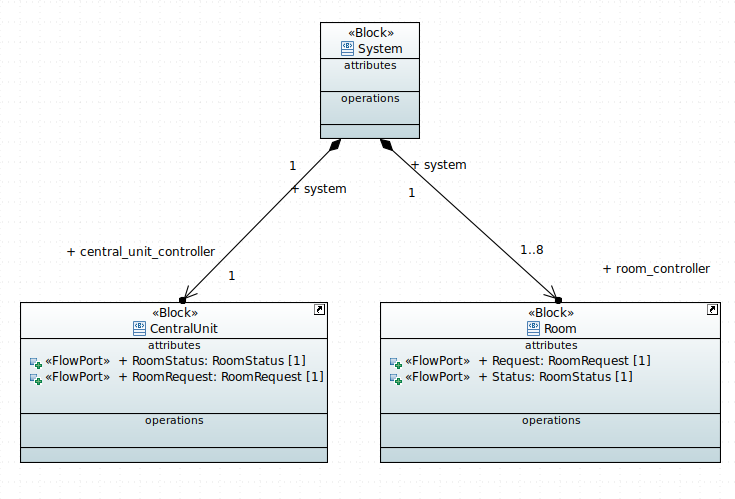
\includegraphics[width=12cm,keepaspectratio]{img/sysml/SystemComponents}
	\caption{System Components}
	\label{fig:SystemComponents}
\end{figure}
\begin{figure}[H]
	\centering
	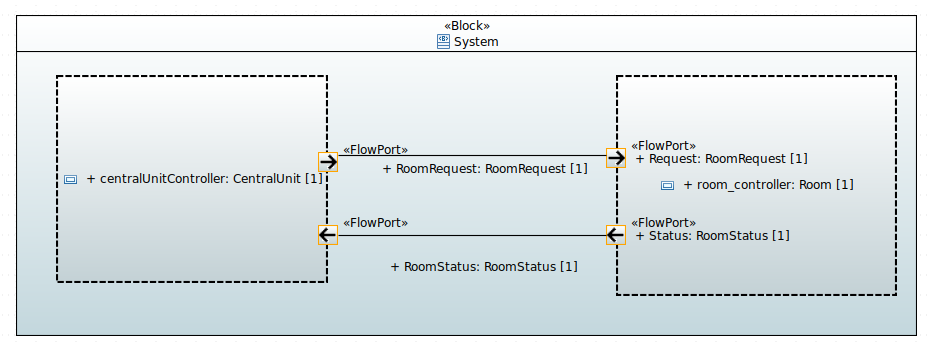
\includegraphics[width=12cm,keepaspectratio]{img/sysml/SystemInternals}
	\caption{System Internals}
	\label{fig:SystemInternals}
\end{figure}

\subsection{Central Unit}
The \textit{Central Unit} is composed by two modules, the \textit{RoomsManager} and the \textit{UserInterfaceManager}.
The \textit{RoomsManager} implements the functionalities related to the status of each room.
The \textit{UserInterfaceManager} that implements the functionalities related to represent the status of the system.
The two components exchange data as shown in \ref{fig:CentralUnit_internals}.
\begin{figure}[H]
	\centering
	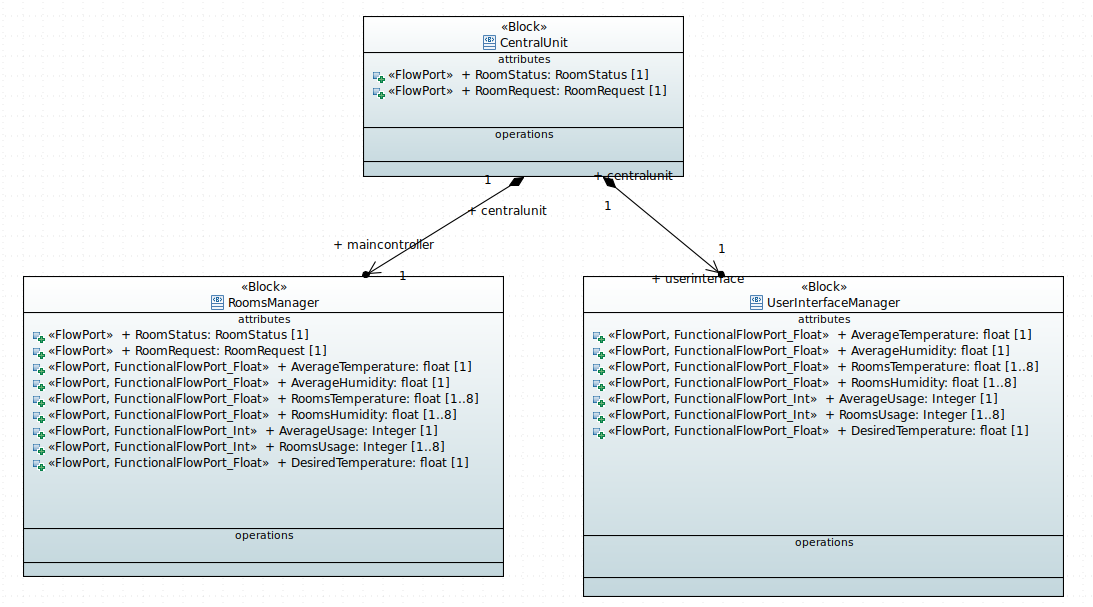
\includegraphics[width=12cm,keepaspectratio]{img/sysml/CentralUnitComponents}
	\caption{Central Unit components}
	\label{fig:CentralUnit_components}
\end{figure}

\begin{figure}[H]
	\centering
	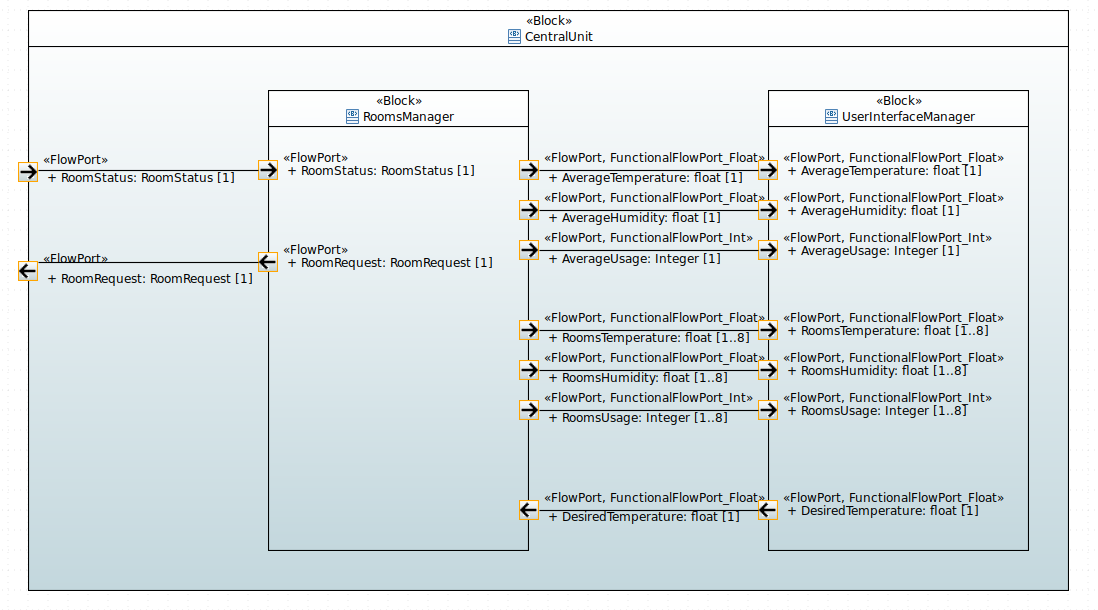
\includegraphics[width=12cm,keepaspectratio]{img/sysml/CentralUnitInternals}
	\caption{Central Unit internals}
	\label{fig:CentralUnit_internals}
\end{figure}

\subsection{Room module}
The main component of this module is the \textit{MainController} composed by different functions as shown in \ref{fig:RoomInternals}.
\begin{figure}[H]
	\centering
	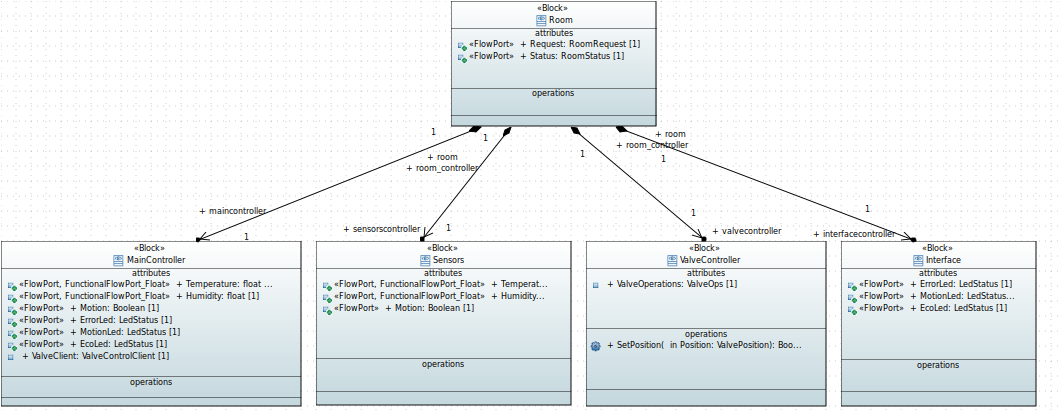
\includegraphics[width=13cm,keepaspectratio]{img/sysml/RoomComponents}
	\caption{Room Components}
	\label{fig:RoomComponents}
\end{figure}

\begin{figure}[H]
	\centering
	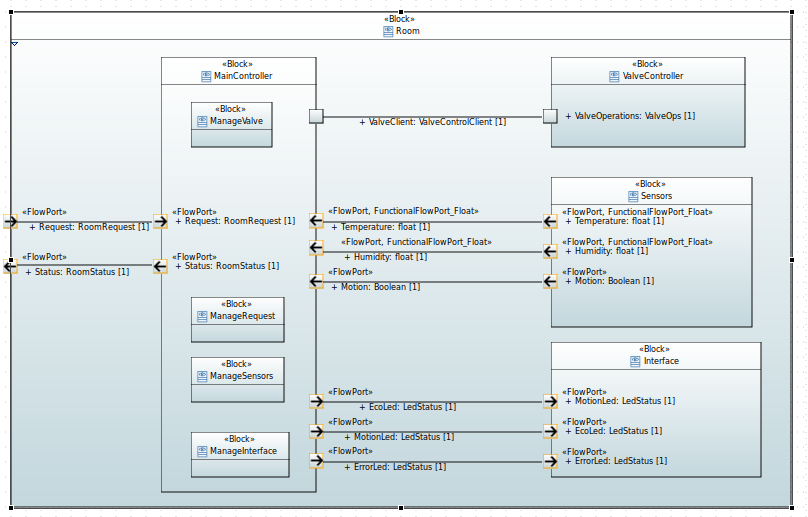
\includegraphics[width=13cm,keepaspectratio]{img/sysml/RoomInternals}
	\caption{Room Internals}
	\label{fig:RoomInternals}
\end{figure}

\begin{figure}[H]
	\centering
	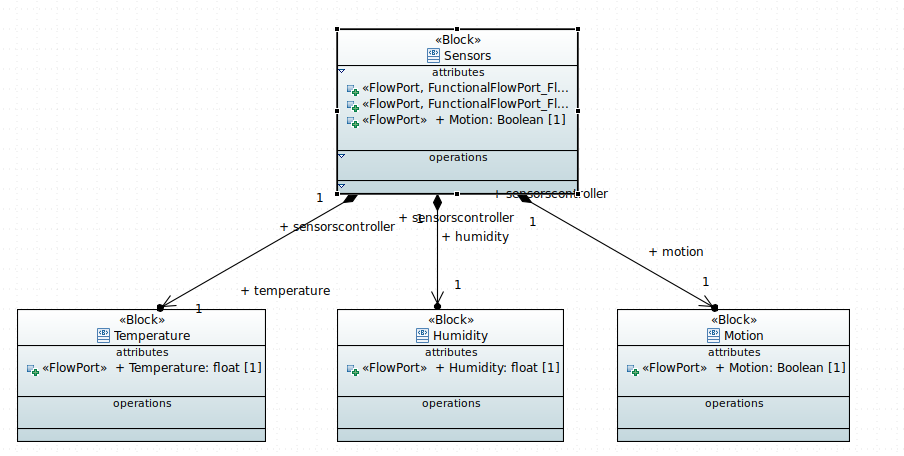
\includegraphics[width=13cm,keepaspectratio]{img/sysml/SensorsComponents}
	\caption{Room sensors components}
	\label{fig:room_sensors_components}
\end{figure}

\begin{figure}[H]
	\centering
	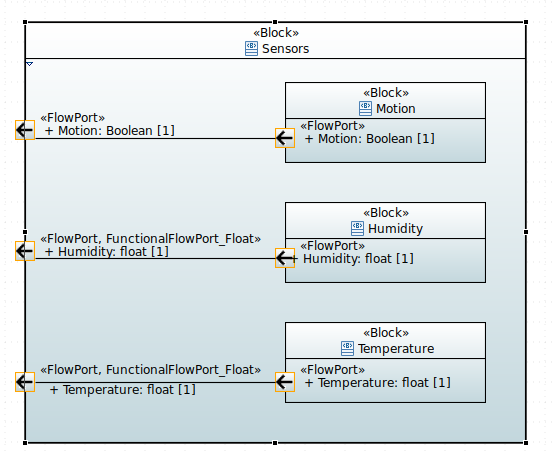
\includegraphics[width=8cm,keepaspectratio]{img/sysml/SensorsInternals}
	\caption{Room sensors internals}
	\label{fig:room_sensors_internals}
\end{figure}

\begin{figure}[H]
	\centering
	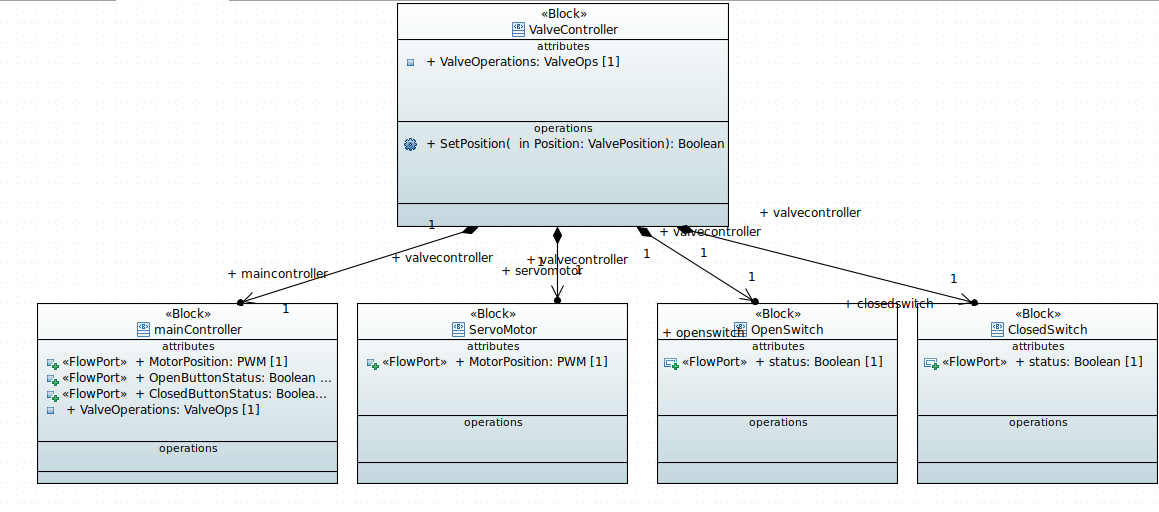
\includegraphics[width=12cm,keepaspectratio]{img/sysml/ValveControllerComponents}
	\caption{Valve Controller components}
	\label{fig:valve_dbd}
\end{figure}

\begin{figure}[H]
	\centering
	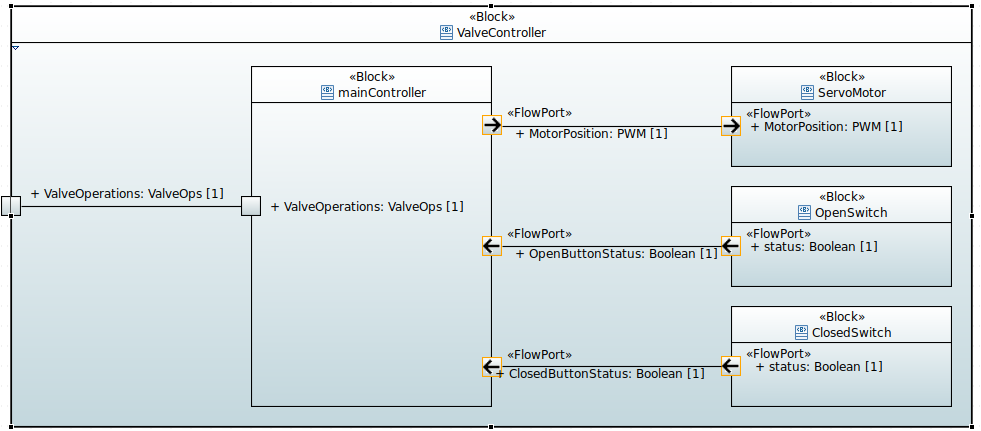
\includegraphics[width=12cm,keepaspectratio]{img/sysml/ValveControllerInternals}
	\caption{Valve Controller internals}
	\label{fig:valve_internals}
\end{figure}

\subsection{Communication State Machines}
In the following pictures are illustrated the behaviour of the communication between the \textit{CentralUnit} and the \textit{Room}.

\begin{figure}[H]
	\centering
	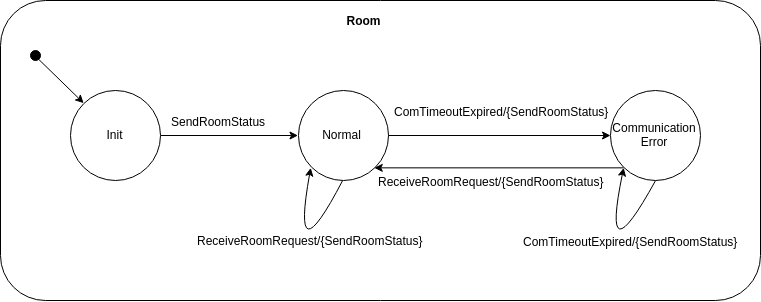
\includegraphics[width=12cm,keepaspectratio]{img/Com_SM_Room}
	\caption{Room communication management}
	\label{fig:room_com}
\end{figure}

In the figure \ref{fig:CU_com_receiver} is described the behaviour of the receiver part in the \textit{CentralUnit}, for readibility is reported just the case of a paramentric room X.\\

In the figure \ref{fig:CU_com_sender} is described the behaviour of the sender part in the \textit{CentralUnit}, for readibility is reported just the case of 2 rooms.

\begin{figure}[H]
	\centering
	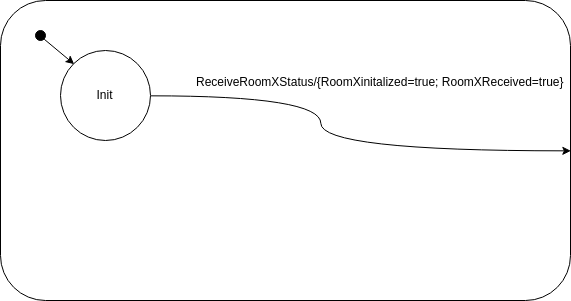
\includegraphics[width=10cm,keepaspectratio]{img/Com_SM_CU_Receiver}
	\caption{Central Unit communication receiver management}
	\label{fig:CU_com_receiver}
\end{figure}

\begin{figure}[H]
	\centering
	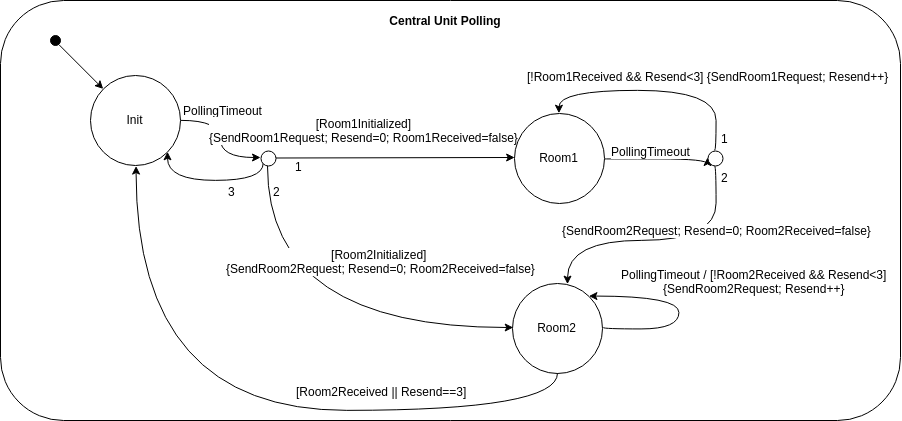
\includegraphics[width=12cm,keepaspectratio]{img/Com_SM_CU_Sender}
	\caption{Central Unit communication sender management}
	\label{fig:CU_com_sender}
\end{figure}


\end{document}